\documentclass{beamer}

\usetheme[sectionpage=simple, subsectionpage=simple,
numbering=fraction, progressbar=none]
{metropolis}

\usepackage[utf8]{inputenc}
\usepackage{graphicx}
\graphicspath{{./img/}}
\usepackage{tikz}

\title{Continuous Random Variables}
\date{\today}
\author{Gonzalo G. Peraza Mues}
% \institute{Universidad Politécnica de Yucatán}

\titlegraphic{
\includegraphics[height=1.5cm]{logo-upy}}

\newcommand{\E}{\operatorname{E}}
\newcommand{\Var}{\operatorname{Var}}
\renewcommand{\P}[1]{P\left(#1\right)}


\begin{document}
\maketitle

\begin{frame}{Definition: Continuous Random Variable}
  A random variable $X$ is \alert{continuous} if it can take on an uncountable
  infinite number of possible outcomes.

  \begin{itemize}
  \item The probability of $X$ taking any \alert{definite} value is exactly
    zero, otherwise the sum of all probabilities would diverge.
  \item The probability that the possible values lie in some fixed
    \alert{interval} $[a, b]$ is the probability we are interested in.
  \end{itemize}
\end{frame}

\begin{frame}{The probability density function}
  \begin{align*}
    P(a\leq X  \leq b) = \int_a^b f(x)dx
  \end{align*}

  \begin{center}
    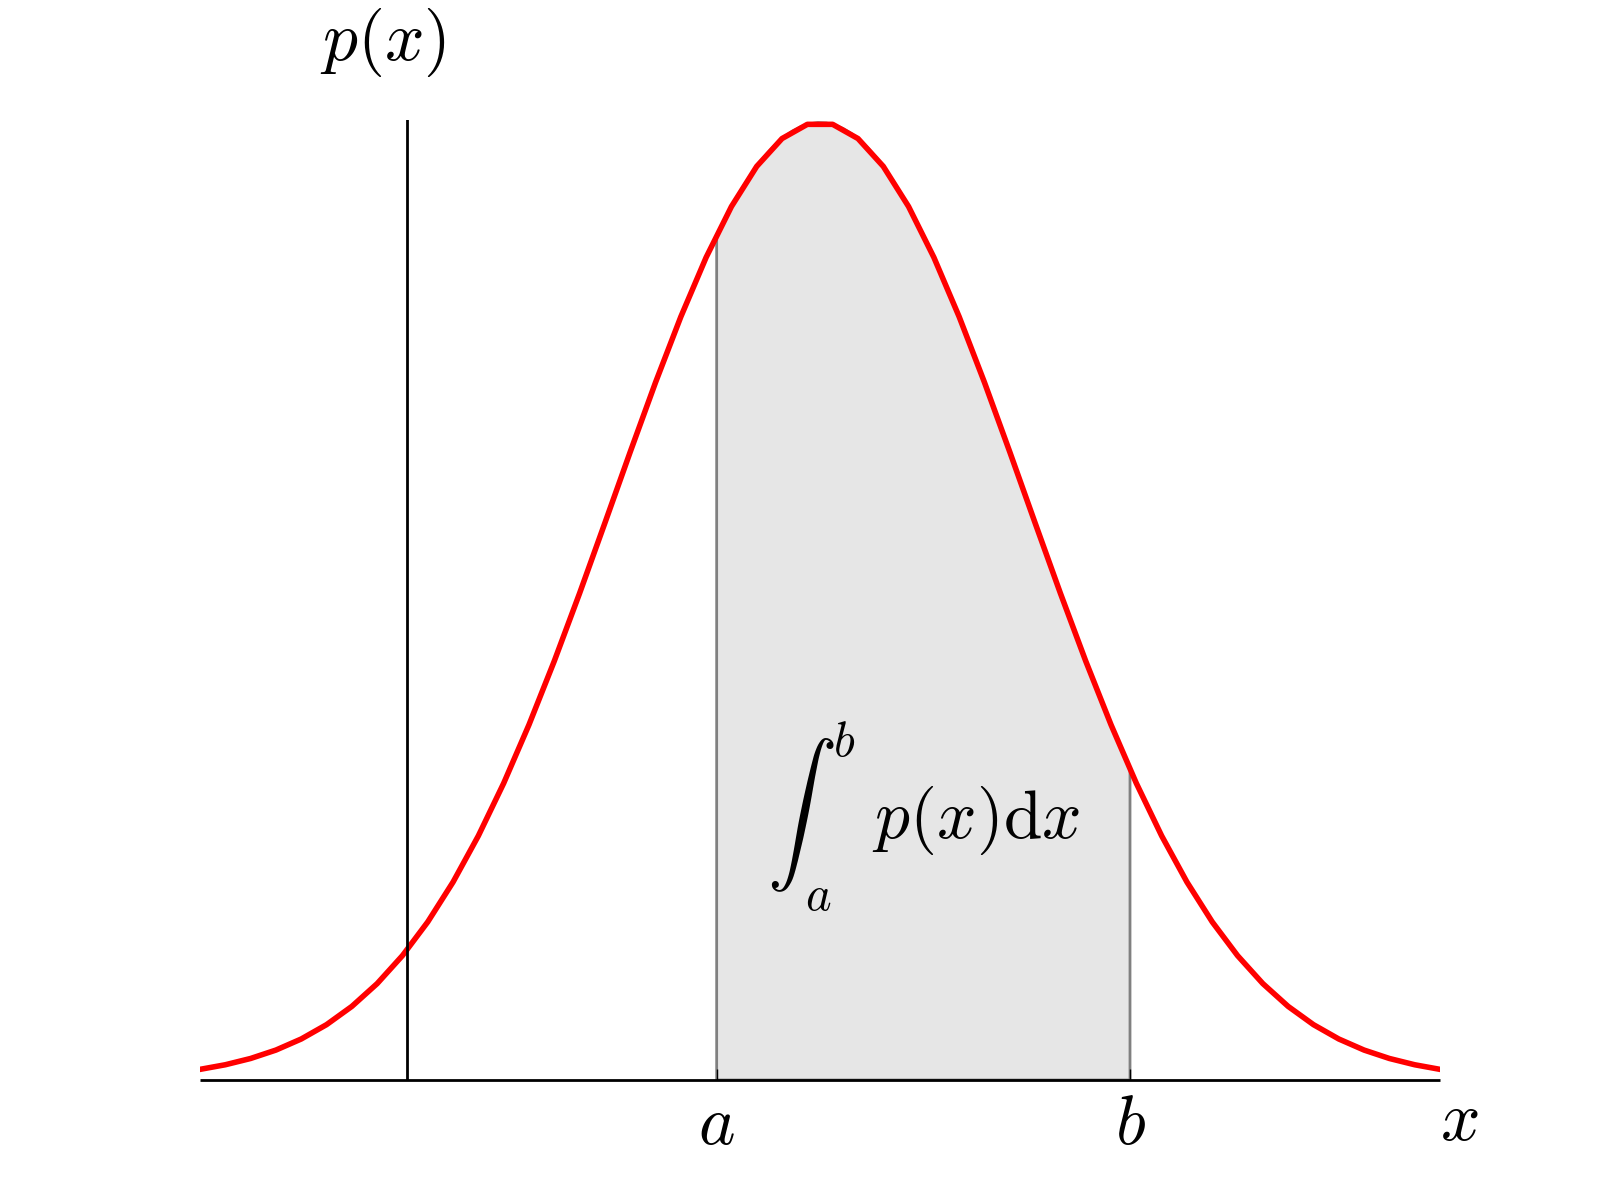
\includegraphics[width=0.7\linewidth]{PDF}
  \end{center}
\end{frame}

\begin{frame}{Properties of $f(x)$}
  \begin{itemize}
  \item $f(x) > 0$ for all $x$
  \item $\int_{-\infty}^\infty f(x)dx = 1$
  \item $f(a)$ is not a probability, it can be interpreted as a (relative)
    measure of how likely it is that $X$ will be near $a$.
  \end{itemize}
\end{frame}

\begin{frame}{The distribution function}
  \begin{align*}
    F(a) = P(X \leq a)
  \end{align*}

  The relation between the probability density function $f$ and the distribution
  function $F$:
  \begin{align*}
    F(b) &= \int_{-\infty}^b f(x)dx\\
    f(x) &= \frac{d}{dx}F(x)
  \end{align*}

  Also, for both discrete and continuous random variables:
  \begin{align*}
    P(a < X \leq b) = P(X \leq b) - P(X \leq a) = F (b) - F (a)
  \end{align*}
\end{frame}

\begin{frame}[t]{The darts example}
  Let $X$ be the distance between the hitting point and the center of the
  disc. Find $P(0<X\leq r/2)$ and $P(r/2<X\leq r)$

  \begin{align*}
    F(b) &= P(X \leq b) = \frac{\pi b^2}{\pi r^2} = \frac{b^2}{r^2}\quad
           \text{for }0\leq b \leq r\\
    f(x) &= \frac{d}{dx}F(x) = \frac{1}{r^2}\frac{d}{dx}x^2=\frac{2x}{r^2}
  \end{align*}
  
\includegraphics[width=0.3\linewidth]{darts}
\end{frame}

\begin{frame}{Expectation and variance}
  \begin{align*}
    E[X] &= \int_{-\infty}^{\infty} xf(x)dx'\\
    Var(X) &= E[{(X - E[X])}^2] = E[X^2] - E[X]^2
  \end{align*}
  The same properties as with discrete random variables apply.
\end{frame}
\begin{frame}{The uniform distribution $U(a,b)$}
  \begin{columns}
    \begin{column}{0.5\textwidth}
      \begin{align*}
        f(x) =
        \begin{cases}
          \frac{1}{b - a} & a \leq x\leq b\\
          0 & \text{otherwise}
        \end{cases}
      \end{align*}
      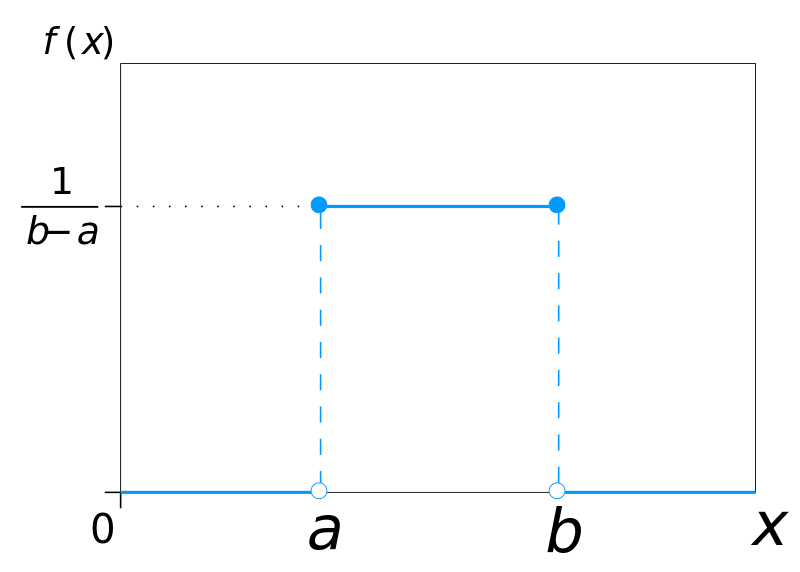
\includegraphics[width=\linewidth]{uniform-pdf}
    \end{column}
    \begin{column}{0.5\textwidth}
      \begin{align*}
        F(x) =
        \begin{cases}
          0 & x < a\\
          \frac{x - a}{b - a} & a \leq b\\
          1 & x > b
        \end{cases}
      \end{align*}
      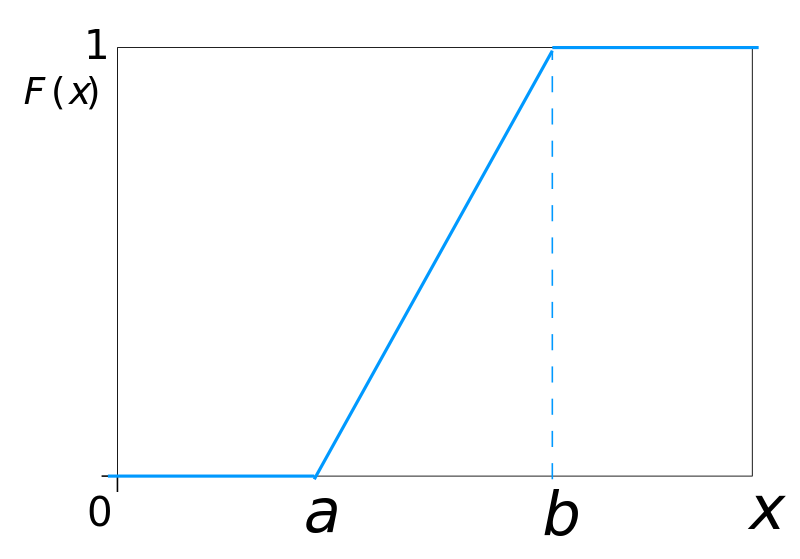
\includegraphics[width=\linewidth]{uniform-df}
    \end{column}
  \end{columns}
  \begin{align*}
    \E[X]=\frac{a+b}{2}\quad\quad\quad\Var(X)=\frac{{(b-a)}^2}{12}
  \end{align*}
\end{frame}

\begin{frame}[t]{The uniform distribution $U(a,b)$. Example}
  Buses arrive at a specified stop at 15-minute intervals starting at 7
  A.M. That is, they arrive at 7, 7:15, 7:30, 7:45, and so on. If a passenger
  arrives at the stop at a time that is uniformly distributed between 7 and
  7:30, find the probability that he waits (a) less than 5 minutes for a bus;
  (b) at least 12 minutes for a bus.


\end{frame}

\begin{frame}{The exponential distribution $Exp(\lambda)$}
  The exponential distribution describes the time for a continuous process to
  change state.
  \begin{itemize}
  \item The time until a radioactive particle decays, or the time between clicks
    of a geiger counter.
  \item The time it takes before your next telephone call.
  \item Distance between roadkills on a given road.
  \end{itemize}
\end{frame}

\begin{frame}{The exponential distribution $Exp(\lambda)$}
  \begin{columns}
    \begin{column}{0.5\textwidth}
      \begin{align*}
        f(x) =
        \begin{cases}
          \lambda e^{-\lambda x} & x \geq 0 \\
          0 & x < 0
        \end{cases}
      \end{align*}
    \end{column}
    \begin{column}{0.5\textwidth}
      \begin{align*}
        F(x) =
        \begin{cases}
          1 - e^{-\lambda x} & x \geq 0\\
          0 & x < b
        \end{cases}
      \end{align*}
    \end{column}
  \end{columns}
  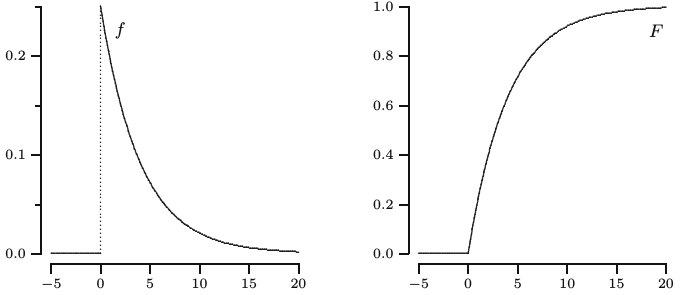
\includegraphics[width=\linewidth]{exp-pdf}
  \begin{align*}
    \E[X]=\lambda^{-1}\quad\quad\quad\Var(X)=\lambda^{-2}
  \end{align*}
\end{frame}

\begin{frame}[t]{Example}
  A study of the response time of a certain computer system yields that the
  response time in seconds has an exponentially distributed time with parameter
  0.25. What is the probability that the response time exceeds 5 seconds?
\end{frame}

\begin{frame}{The normal distribution $N(\mu,\sigma^2)$}
  \begin{columns}
    \begin{column}{0.5\textwidth}
      \begin{align*}
        f(x) = \frac{1}{\sigma\sqrt{2\pi}}
        e^{-\frac{1}{2}{\left(\frac{x-\mu}{\sigma}\right)}^2}
      \end{align*}
    \end{column}
    \begin{column}{0.5\textwidth}
      \begin{align*}
        F(a) = \int_{-\infty}^a \frac{1}{\sigma\sqrt{2\pi}}
        e^{-\frac{1}{2}{\left(\frac{x-\mu}{\sigma}\right)}^2}dx
      \end{align*}
    \end{column}
  \end{columns}
  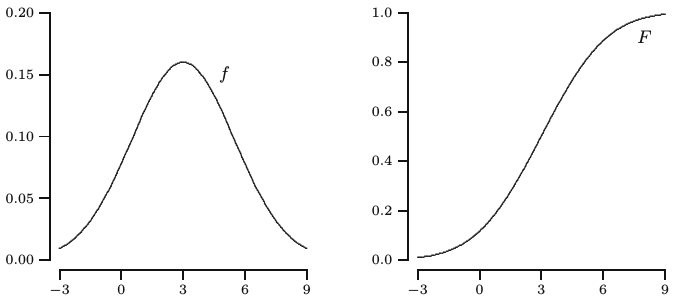
\includegraphics[width=\linewidth]{normal-pdf}
  \begin{align*}
    \E[X]=\mu\quad\quad\quad\Var(X)=\sigma^2
  \end{align*}
\end{frame}

\begin{frame}{The normal distribution $N(\mu,\sigma^2)$}
  Some examples of this behavior are the height of a person, the velocity in any
  direction of a molecule in gas, and the error made in measuring a physical
  quantity.

  If X is normal with mean $\mu$ and variance $\sigma^2$, then for any constants
  $a$ and $b$, $b\ne 0$, the random variable $Y = a +bX$ is also a normal random
  variable with parameters
  \begin{align*}
    \E[Y] =& a + b\mu\\
    \Var(Y) =& b^2\sigma^2
  \end{align*}

\end{frame}

\begin{frame}{The normal distribution $N(\mu,\sigma^2)$}
  Any $N (\mu, \sigma^2)$ distributed random variable can be turned into an
  $N(0,1)$ distributed random variable by a simple transformation:

  \begin{align*}
    Z=\frac{X-\mu}{\sigma}
  \end{align*}

  This yields the standard normal distribution $\phi$:
  \begin{align*}
    \phi (x) = \frac{1}{\sqrt{2\pi}}
    e^{-\frac{1}{2}{x}^2}
  \end{align*}
  with an associated distribution function:
  \begin{align*}
    \Phi (x) = \int_{-\infty}^x \frac{1}{\sqrt{2\pi}}
    e^{-\frac{1}{2}{y}^2}dy
  \end{align*}
\end{frame}

\begin{frame}{The normal distribution $N(\mu,\sigma^2)$}
  \begin{align*}
    P(X<b) =& \Phi\left(\frac{b-\mu}{\sigma}\right) \\
    P(a<X<b) =& \Phi\left(\frac{b-\mu}{\sigma}\right) -
                \Phi\left(\frac{a-\mu}{\sigma}\right)\\
    \Phi(-x) =& 1 - \Phi(x)
  \end{align*}
\end{frame}

\begin{frame}[t]{The normal distribution $N(\mu,\sigma^2)$. Example}
  Let the random variable $Z$ have a standard normal distribution. Use R(pnorm)
  to find $P(Z \leq 0.75)$. How do you know, without doing any calculations,
  that the answer should be larger than 0.5?
\end{frame}

\begin{frame}[t]{The normal distribution $N(\mu,\sigma^2)$. Example}
  If X is a normal random variable with mean $\mu = 3$ and variance
  $\sigma^2 = 16$, find (a) $\P{X < 11}$; (b) $\P{X > -1}$; (c) $\P{2 < X < 7}$.
\end{frame}

\begin{frame}{The normal distribution $N(\mu,\sigma^2)$}
  The sum of independent normal random variables is also a normal random
  variable.

  $\sum_{i=1}^n X_i$ is normal with mean $\sum_{i=1}^n \mu_i$ and variance
  $\sum_{i=1}^n \sigma_i^2$.
\end{frame}
\begin{frame}[t]{The normal distribution $N(\mu,\sigma^2)$. Example}
  Data from the National Oceanic and Atmospheric Administration indicate that
  the yearly precipitation in Los Angeles is a normal random variable with a
  mean of 12.08 inches and a standard deviation of 3.1 inches. (a) Find the
  probability that the total precipitation during the next 2 years will exceed
  25 inches. (b) Find the probability that next year’s precipitation will exceed
  that of the following year by more than 3 inches.


\end{frame}
\begin{frame}{The Chi-Square Distribution}
  If $Z_1,Z_2 ,\ldots,Z_n$ are independent standard normal random variables,
  then
  \begin{align*}
    X = Z_1^2 + Z_2^2 + \cdots + Z_n^2
  \end{align*}
  is said to have a chi-square distribution with n degrees of freedom. We will
  use the notation $X \sim \chi_n^2$ to signify that X has a chi-square distribution with
  n degrees of freedom.
\end{frame}

\begin{frame}{The Chi-Square Distribution}
  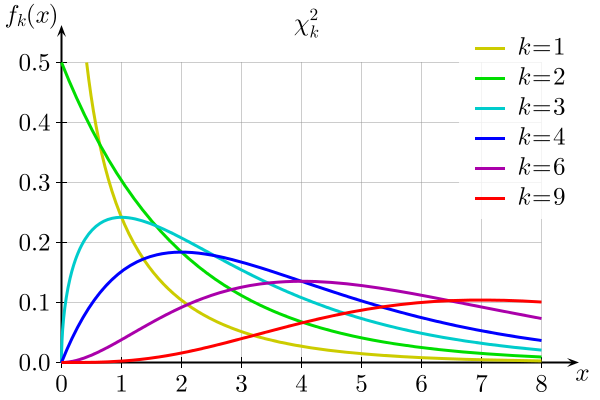
\includegraphics[width=0.8\linewidth]{Chi-square_pdf}
\end{frame}

\begin{frame}{The Chi-Square Distribution}
  If $X_1$ and $X_2$ are independent chi-square random variables with $n_1$ and
  $n_2$ degrees of freedom, respectively, then $X_1 + X_2$ is chi-square with
  $n_1 + n_2$ degrees of freedom.
\end{frame}

\begin{frame}{The Chi-Square Distribution}
  If X is a chi-square random variable with n degrees of freedom, then for any
  $\alpha \in (0, 1)$, the quantity $\chi_{\alpha,n}^2$ is defined to be such
  that
  \begin{align*}
    \P{X \geq \chi_{\alpha,n}^2 }= \alpha
  \end{align*}
  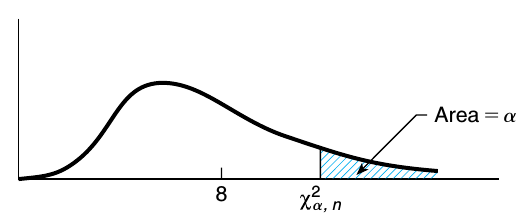
\includegraphics[width=\linewidth]{chi-alpha-n}
\end{frame}

\begin{frame}[t]{The Chi-Square Distribution. Example}
  Determine $\P{\chi_{26}^2 \leq 30}=0.732$ (Use the R function pchisq)

  Find $\chi_{0.05,15}^2=24.996$ (Use the R function qchisq)

  Suppose that we are attempting to locate a target in three-dimensional space,
  and that the three coordinate errors (in meters) of the point chosen are
  independent normal random variables with mean 0 and standard deviation 2. Find
  the probability that the distance between the point chosen and the target
  exceeds 3 meters.

\end{frame}

\begin{frame}{The t-Distribution}
  If Z and $\chi_n^2$ are independent random variables, with Z having a standard
  normal distribution and $\chi_n^2$ having a chi-square distribution with n
  degrees of freedom, then the random variable $T_n$ defined by
  \begin{align*}
    T_n = \frac{Z}{\sqrt{\chi_n^2/n}}
  \end{align*}
  is said to have a t-distribution with n degrees of freedom.

  For let $t_{\alpha,n}$ be such that $\P{T_n \geq t_{\alpha,n} } = \alpha$
\end{frame}

\begin{frame}{The t-Distribution}
  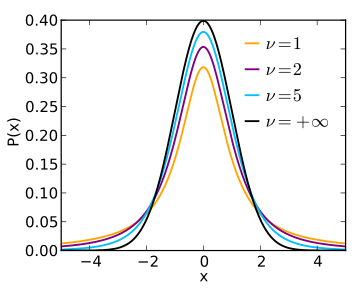
\includegraphics[width=0.8\linewidth]{Student_t_pdf}
  \begin{align*}
    \E[T_n] = 0 \quad \Var(T_n) = \frac{n}{n-2}
  \end{align*}
\end{frame}

\begin{frame}[t]{The t-Distribution. Example}
  Find (a) $\P{T_{12} \leq 1.4}=0.9066$ and (b) $t_{0.025,9}=2.2621$. (Use R
  functions pt and qt)
\end{frame}

\begin{frame}{The F-Distribution}
  If $\chi_n^2$ and $\chi_m^2$ are independent chi-square random variables with
  n and m degrees of freedom, respectively, then the random variable $F_{n,m}$
  defined by
  \begin{align*}
    F_{n,m} = \frac{\chi_n^2/n}{\chi_m^2/m}
  \end{align*}
  is said to have an F-distribution with n and m degrees of freedom.

  Let $F_{\alpha,n,m}$ be such that $\P{F_{n,m} > F{\alpha,n,m} } = \alpha$.

  Example: Determine $\P{F_{6,14} \leq 1.5} = 0.7518$ (Use the R function pf).
\end{frame}

\end{document}

%%% Local Variables:
%%% mode: latex
%%% TeX-master: t
%%% End:
